
The rapid steady-state \gls{MRI} sequences are a sub-category of fast gradient-echo sequences where the excitation pulses are applied consecutively at a constant but much faster rate than the longitudinal and transverse relaxation times $(T_1, T_2 << TR)$. In addition to enabling fast imaging, the signal dependence on the previous excitations generates novel structural and functional contrast mechanism. Depending on whether the transverse magnetization is spoiled/excluded after each repetition, the steady-state methods can be classified into steady-state incoherent and coherent methods as shown in \cref{fig:ss_seq}. The incoherent methods such as \gls{FLASH} \cite{haaseFLASHImagingRapid1986}/\gls{SPGR} eliminate the residual transverse magnetization before the next excitation with gradient spoiling and quadratic \gls{RF} phase increments known as \gls{RF} spoiling. Despite the first rapid steady state method \gls{FLASH} being proposed later than existing gradient-echo \gls{EPI} \cite{mansfieldMultiplanarImageFormation1977} and spin-echo \gls{RARE} \cite{hennigRAREImagingFast1986} methods, it was quickly adopted into clinical routine because of its speed, high image quality, desirable $T_1$ contrast and reliability.
\newline
The coherent methods does not use RF spoiling. Therefore, both longitudinal and transverse components evolve over multiple repetition resulting in a more complicated signal dependence on flip angle, $T_1$, $T_2$ and off-resonance. By carefully adjusting the unbalanced gradient moments, \gls{FID} part of \gls{SSFP} signal with prominent $T_1$ weighting \cite{oppletFISPNewFast1986} or Echo part of \gls{SSFP} signal with prominent $T_2$ weighting \cite{gyngellApplicationSteadystateFree1988} can be acquired. The \gls{SSFP}-\gls{FID} goes by several acronyms in literature and by vendors such as $F_0$, $S+$, \gls{FISP} (Siemens), FAST (GE), FFE(Philips). Similarly,  \gls{SSFP}-Echo is known by its alternative names such as $F_{-1}$, $S-$, PSIF (Siemens), CS-FAST (GE) and $T_2$-FFE (Philips). These methods are not widely used in clinics except for some niche applications like multi-parametric mapping \cite{heuleTripleEchoSteadystate2014} because of their undesirable contrast and the availability of better alternatives. Furthermore, the unbalanced gradient makes these methods highly sensitive to flow and motion. There are numerous other unbalanced \gls{SSFP} methods possible with even larger unbalanced gradients such as echo shifted GRE which have only limited application due to the increased motion sensitivity and exponentially decreasing sensitivity with the dephasing order \cite{chungSignalFormationEchoshifted1999, schefflerPictorialDescriptionSteadystates1999}.

The \gls{bSSFP} (True\gls{FISP}, FIESTA or balanced FFE) method \cite{carrSteadyStateFreePrecession1958, zurMotioninsensitiveSteadystateFree1990} is a special case of coherent steady-state sequence where the gradient moment is nulled before each excitation. The gradient moment nulling makes the \gls{bSSFP} acquisition highly motion insensitive and additionally, provides the possibility to simultaneously acquire signal from multiple signal pathways. This improves the \gls{SNR} of bSSFP acquisition and also, makes it more sensitive to additional phase accumulations due to temporal field drifts and spatial $B_0$ off-resonance. Its characteristic $T_2/T_1$ contrast makes it ideal for fluids with an unmatched \gls{SNR} per unit time compared to all other sequence. With the improving scanner hardware, \gls{bSSFP} is finding increasing applications in cardiac imaging, angiography, multi-parametric mapping, and adequate spin-echo contrast replacement in some cases \cite{schefflerPrinciplesApplicationsBalanced2003}. Due the limited scope of this thesis, only the \gls{bSSFP} signal model is introduced in the following subsections.

\begin{figure}[H]
	\centering
	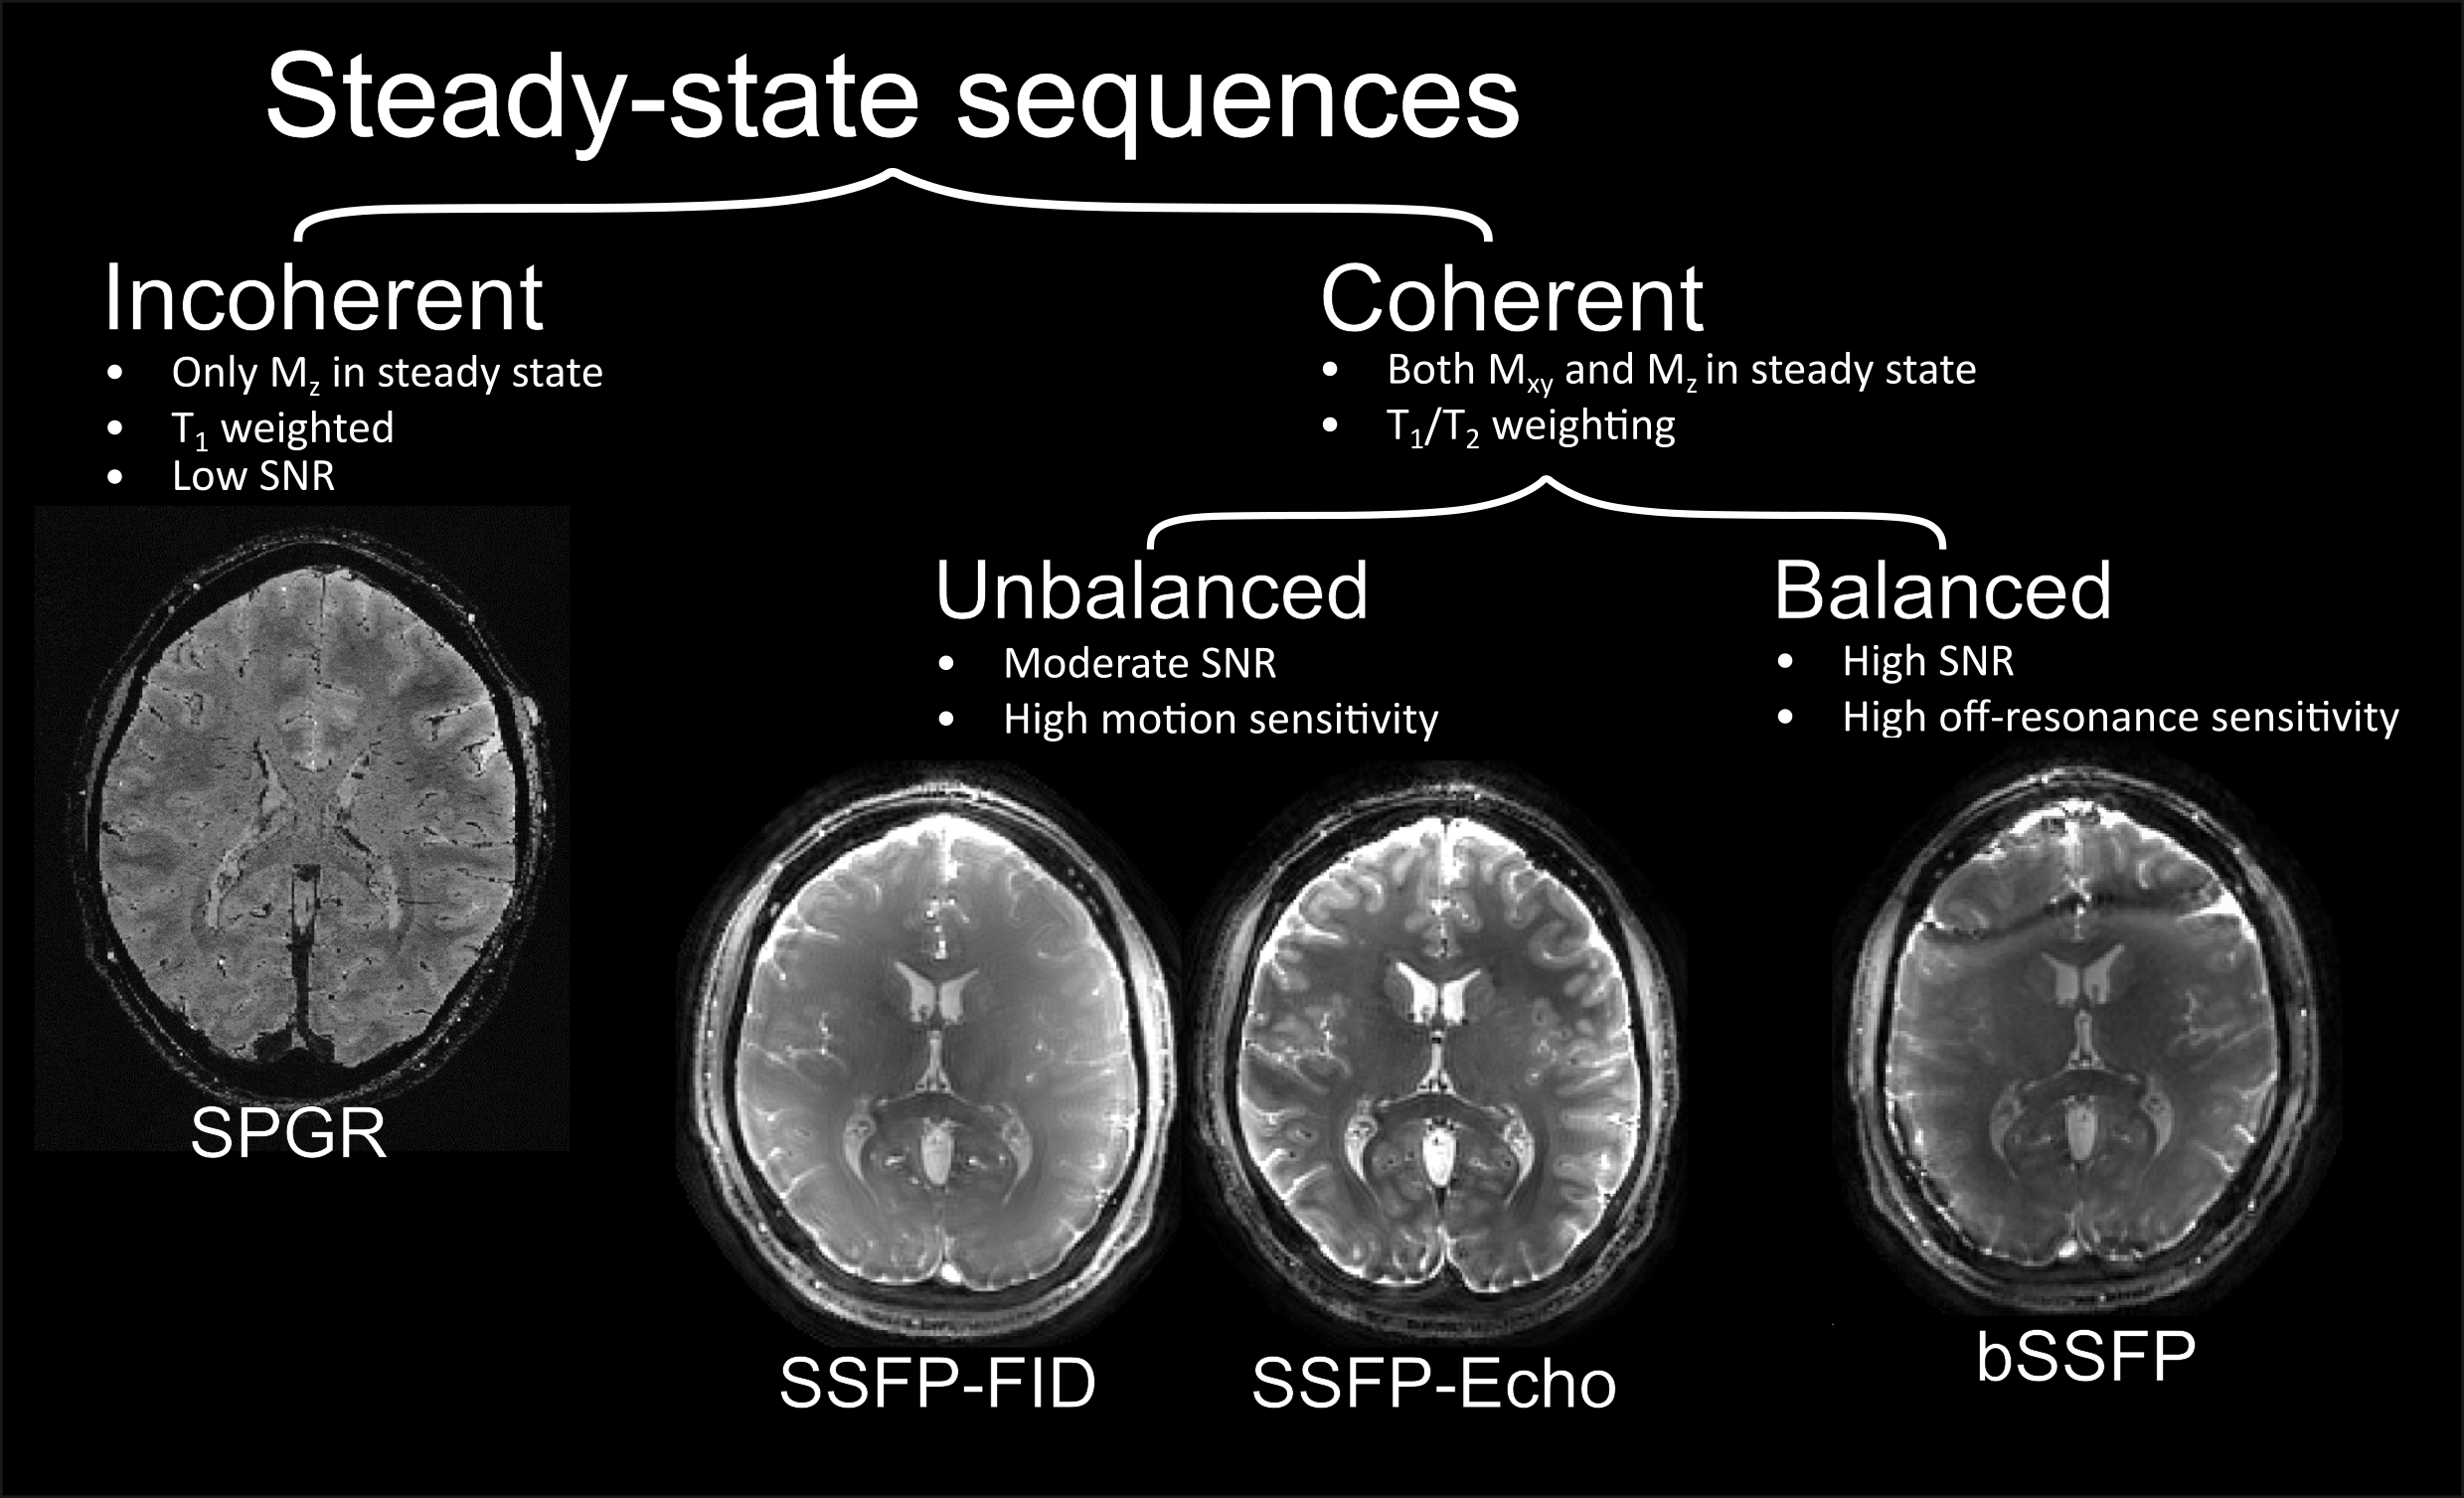
\includegraphics[width=1.0\textwidth]{graphics/ss_seq.png}
	\caption{Classification of steady-state sequences. }
	\label{fig:ss_seq}
\end{figure}

\subsection{Transient phase: the transition to steady-state}
In order to measure the steady-state signal, the magnetization must be brought to the desirable equilibrium condition. Depending on relaxation time, sequence parameters and off-resonance, several repetitions of excitation, relaxation and free precession are required for the magnetization to reach the steady-state \cite{bieriFundamentalsBalancedSteady2013}. Normally, the magnetization will reach steady-state after repetitions with no signal acquisition known as dummy cycles for the duration of $5\cdot T_1$ \cite{schefflerTransientPhaseBalanced2003}. Often this long preparation is impractical. Therefore, short preparation blocks were proposed such as ($\alpha/2$ pulse - TR/2) preparation\cite{deimingMagnetizationPreparedTrue1994}, linear flip angle ramp \cite{nishimuraAnalysisReductionTransient} and optimized preparation block based on eigenvector analysis \cite{hargreavesCharacterizationReductionTransient2001,jaynesMatrixTreatmentNuclear1955}. A shaped flip angle ramp is usually favored for its simplicity and for having a short transient phase with much reduced oscillatory component due to the off-resonant magnetization.    

\subsection{bSSFP frequency response}
In the steady state, a closed-form signal amplitude can be obtained by modeling the periodic nature of the magnetization\cite{jaynesMatrixTreatmentNuclear1955,zurMotioninsensitiveSteadystateFree1990}. The steady-state transverse magnetization $M^+_{\perp}$ for flip angle $\alpha$, relaxation times $T_1$ and $T_2$, and repetition time TR is given by\cite{ganterSteadyStateGradient2006}

\begin{equation}
M^+_{\perp}(\alpha,\theta)=M_0\frac{-i(1-E_1)\sin \alpha (1-E_2e^{-i\theta})}{(1-E_1\cos \alpha)(1+E_2\cos \theta)+(\cos \alpha -E_1)(E_2+ \cos \theta)E_2} 
	\label{eq:bSSFPfreqResponse}	
\end{equation}

With the relaxation terms $E_1 \coloneqq \exp\left(-\frac{TR}{T_{1,j}}\right)$ and  $E_{2} \coloneqq \exp\left(-\frac{TR}{T_2}\right)$ and the phase term $\theta\coloneqq \vartheta- \varphi$ being the phase accumulated by the transverse magnetization during each TR due to off-resonance $\vartheta$ and RF phase increment $\varphi$.

\begin{figure}[H]
	\centering
	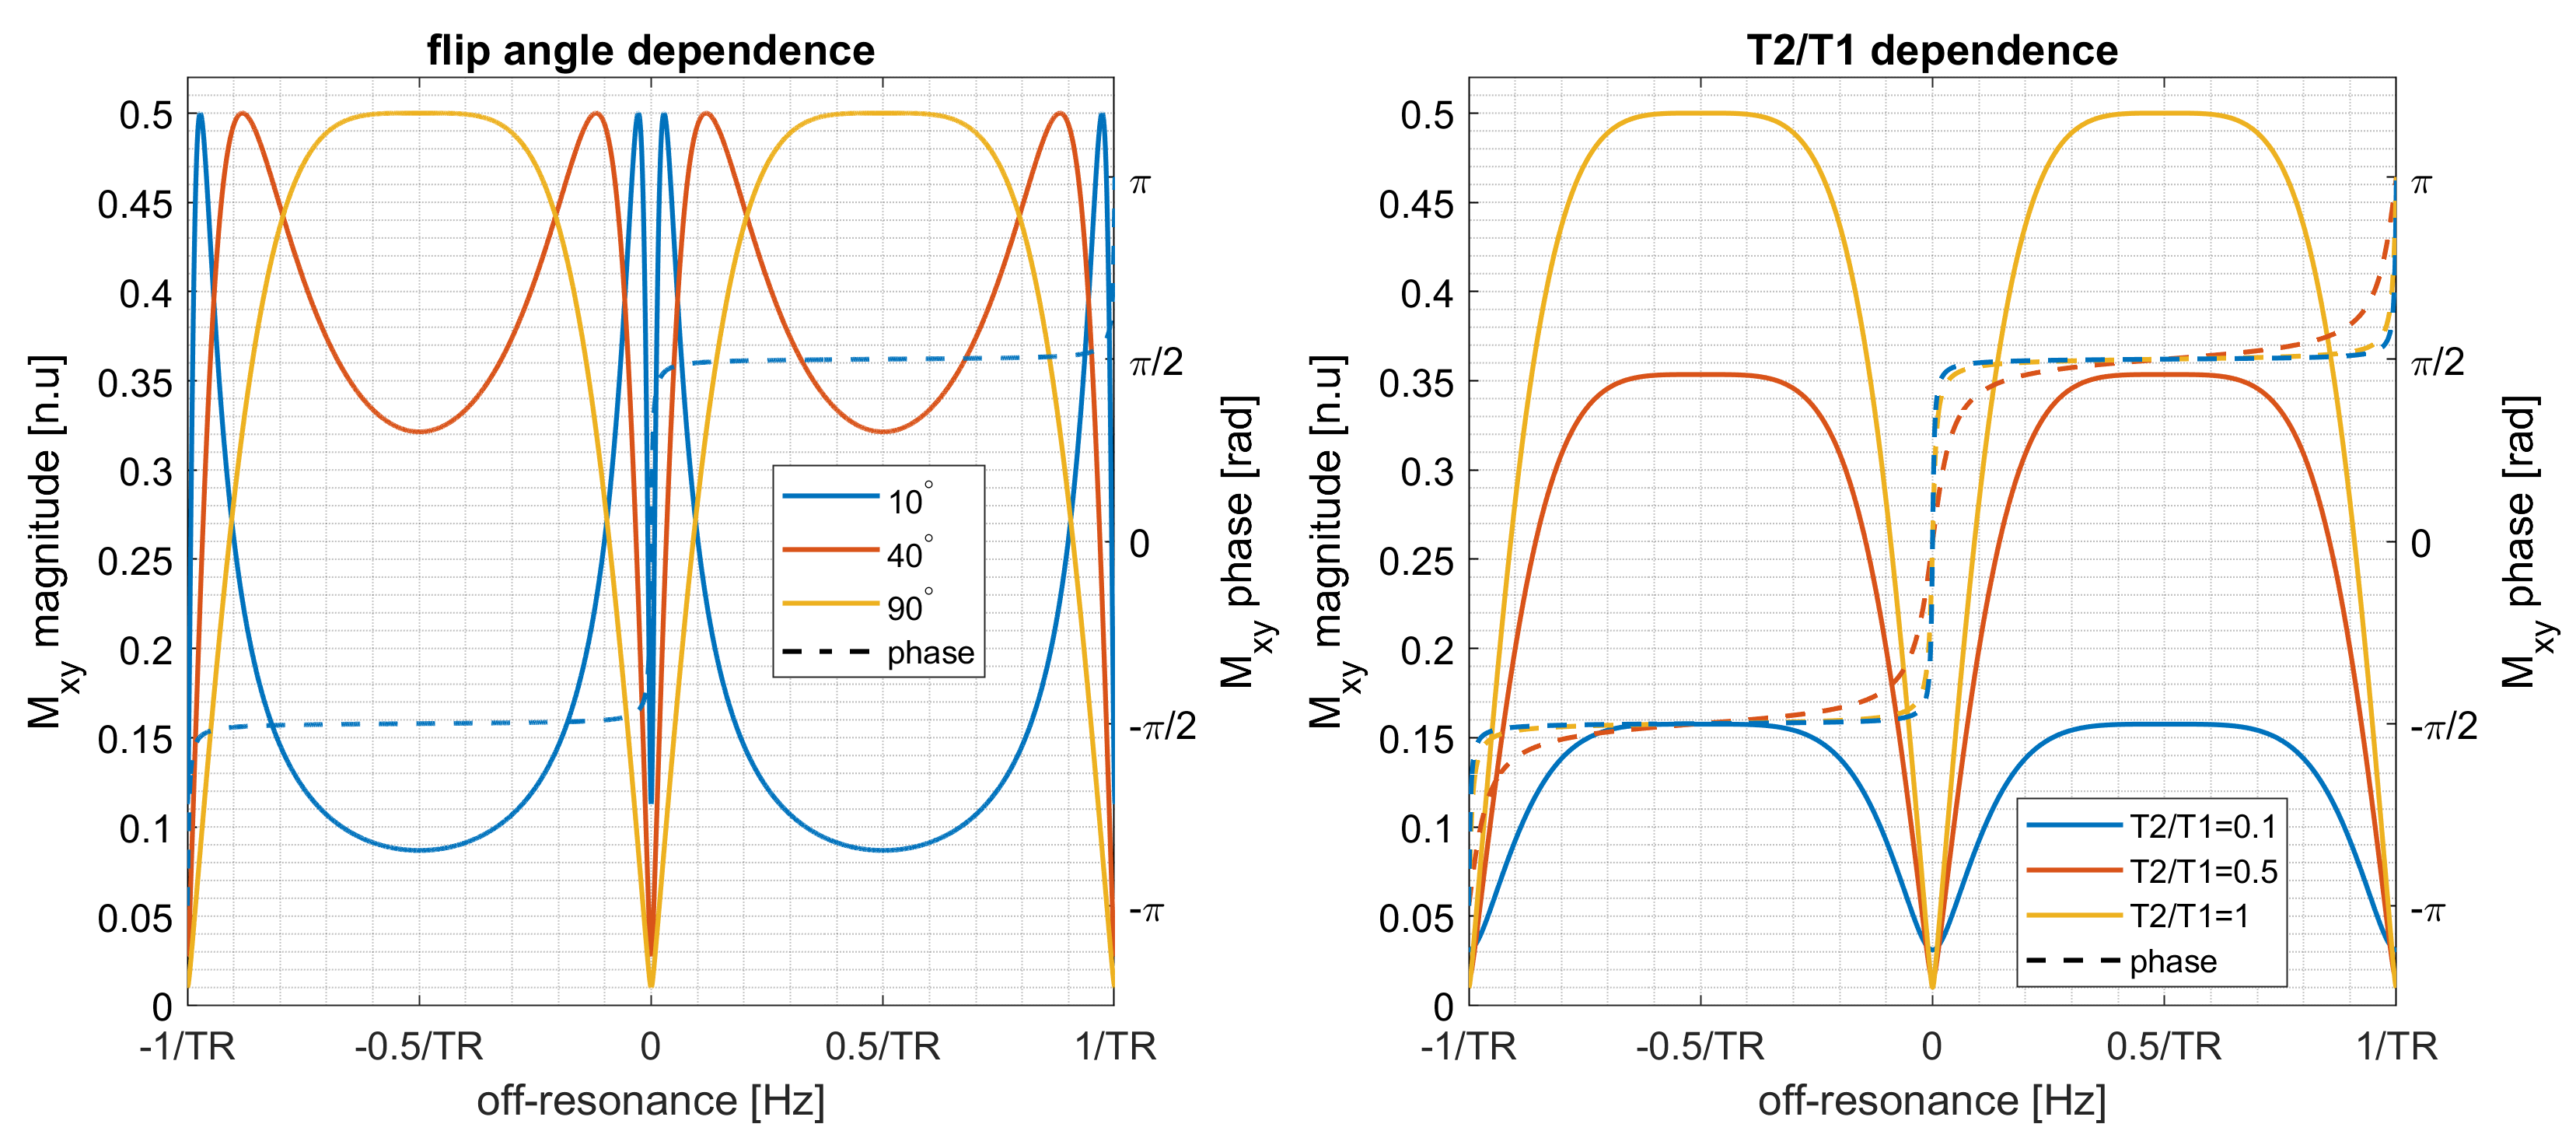
\includegraphics[width=1.0\textwidth]{graphics/bSSFP_freqResponse.png}
	\caption{The \gls{bSSFP} signal dependence on off-resonance, flip angle, and the $T_2/T_1$ ratio. The magnitude (solid) and phase (dashed) of transverse magnetization $M_{xy}$ with respect to off-resonance for three flip angles are shown on the left. The relaxation times are $T_1 = T_2 = 0.5 \, \text{s}$. On the right, the magnitude (solid) and phase (dashed) of transverse magnetization $M_{xy}$ with respect to off-resonance for three $T_2/T_1$ ratios, with $T_1 = 0.5 \, \text{s}$, are presented. The estimated optimal flip angles of $35^\circ$, $70^\circ$, and $90^\circ$ were used for the simulations corresponding to $T_2/T_1$ ratios of 0.1, 0.5, and 1, respectively. The other sequence parameters used for the simulation are TR = 10 ms, TE = TR/2, and, RF phase increment $\varphi=0$.}
	\label{fig:bSSFP_freqresp}
\end{figure}

The steady-state signal of \gls{bSSFP} acquisition exhibits a strong dependence on off-resonance effects, in contrast to gradient or RF-spoiled \gls{GRE} sequences. In addition to off-resonance, the shape of the bSSFP frequency response depends on both flip angle and $T_2/T_1$ ratio, as shown in \cref{fig:bSSFP_freqresp}. Notably, the magnitude part of the bSSFP frequency response is periodic with a period of 1/TR. The regions of high signal within this response are referred to as the passband, which covers about 70\% of the overall frequency response. Conversely, the low signal regions are termed the stopband, which are responsible for banding artifacts commonly observed in bSSFP images. It is worth noting that this behavior is reversed in the low flip angle regime, where the passband and stopband characteristics change. Unlike spoiled acquisition schemes, the optimal flip angle for maximizing passband steady-state signal in bSSFP depends on both $T_1$ and $T_2$ relaxation times\cite{bieriFundamentalsBalancedSteady2013}. The maximum possible transverse magnetization of $0.5\,\cdot\,M_0$ is achieved when $T_1$ and $T_2$ are equal for a flip angle of $90^\circ$. Another interesting feature of the frequency response is the constant phase response to off-resonances less than 1/TR. This behavior bears a striking similarity to the spin-echo technique, where all off-resonances exhibit zero phase at echo time. This intriguing resemblance\cite{schefflerTrueFISPGradientechoSpinecho2003} is used in some niche spin-echo like applications\cite{bowenHighFieldBalancedSSFP2005,schefflerHighresolutionFunctionalImaging2015} where acquisition speed and high energy deposition are of primary concern. It should be noted that the presented bSSFP frequency response is derived from a single isochromat. In an imaging experiment, the distribution of isochromats, as indicated by the intravoxel spectrum, introduces asymmetries\cite{millerAsymmetriesBalancedSSFP2010} and alters the refocusing behavior of bSSFP\cite{ganterStaticSusceptibilityEffects2006}.

\subsection{phase cycling}
The bSSFP imaging experiment is typically conducted under passband conditions, where a linear \gls{RF} phase increment of $\varphi = 180^\circ$ is used to keep on-resonant spins within the passband. Achieving sufficient shimming across the entire imaging volume to avoid banding artifacts is challenging, particularly at high field strengths. Mitigation strategies include (1) shimming only the region of interest, (2) reducing TR to increase the banding-width, and (3) adjusting the system frequency or linear RF phase increment to shift banding regions away from the region of interest. However, when a sufficiently homogeneous static field cannot be achieved, multiple bSSFP acquisitions with different linear RF phase increments can be used to improve coverage. This process is known as phase cycling. The main drawback of phase cycling is the increased acquisition time. Furthermore, the combined images have lower \gls{SNR} and may exhibit different contrast compared to passband \gls{bSSFP} acquisitions, depending on the combination method~\cite{bangerterAnalysisMultipleacquisitionSSFP2004}.
 
\subsection{bSSFP Configuration modes}
It is beneficial to study the \gls{bSSFP} signal with extended phase graph formalism\cite{weigelExtendedPhaseGraphs2015}. The echoes are the coherent transverse magnetization producing observable signal under the influence of multiple RF excitations, gradient dephasing and relaxation cycles\cite{hennigEchoesHowGenerate1991}. As the gradient moment is nulled in between repetitions, the steady-state transverse magnetization is summation of all echo amplitudes as illustrated in \cref{fig:bSSFP_echoes}\cite{zurMotioninsensitiveSteadystateFree1990}. 
 
 \begin{figure}[H]
 	\centering
 	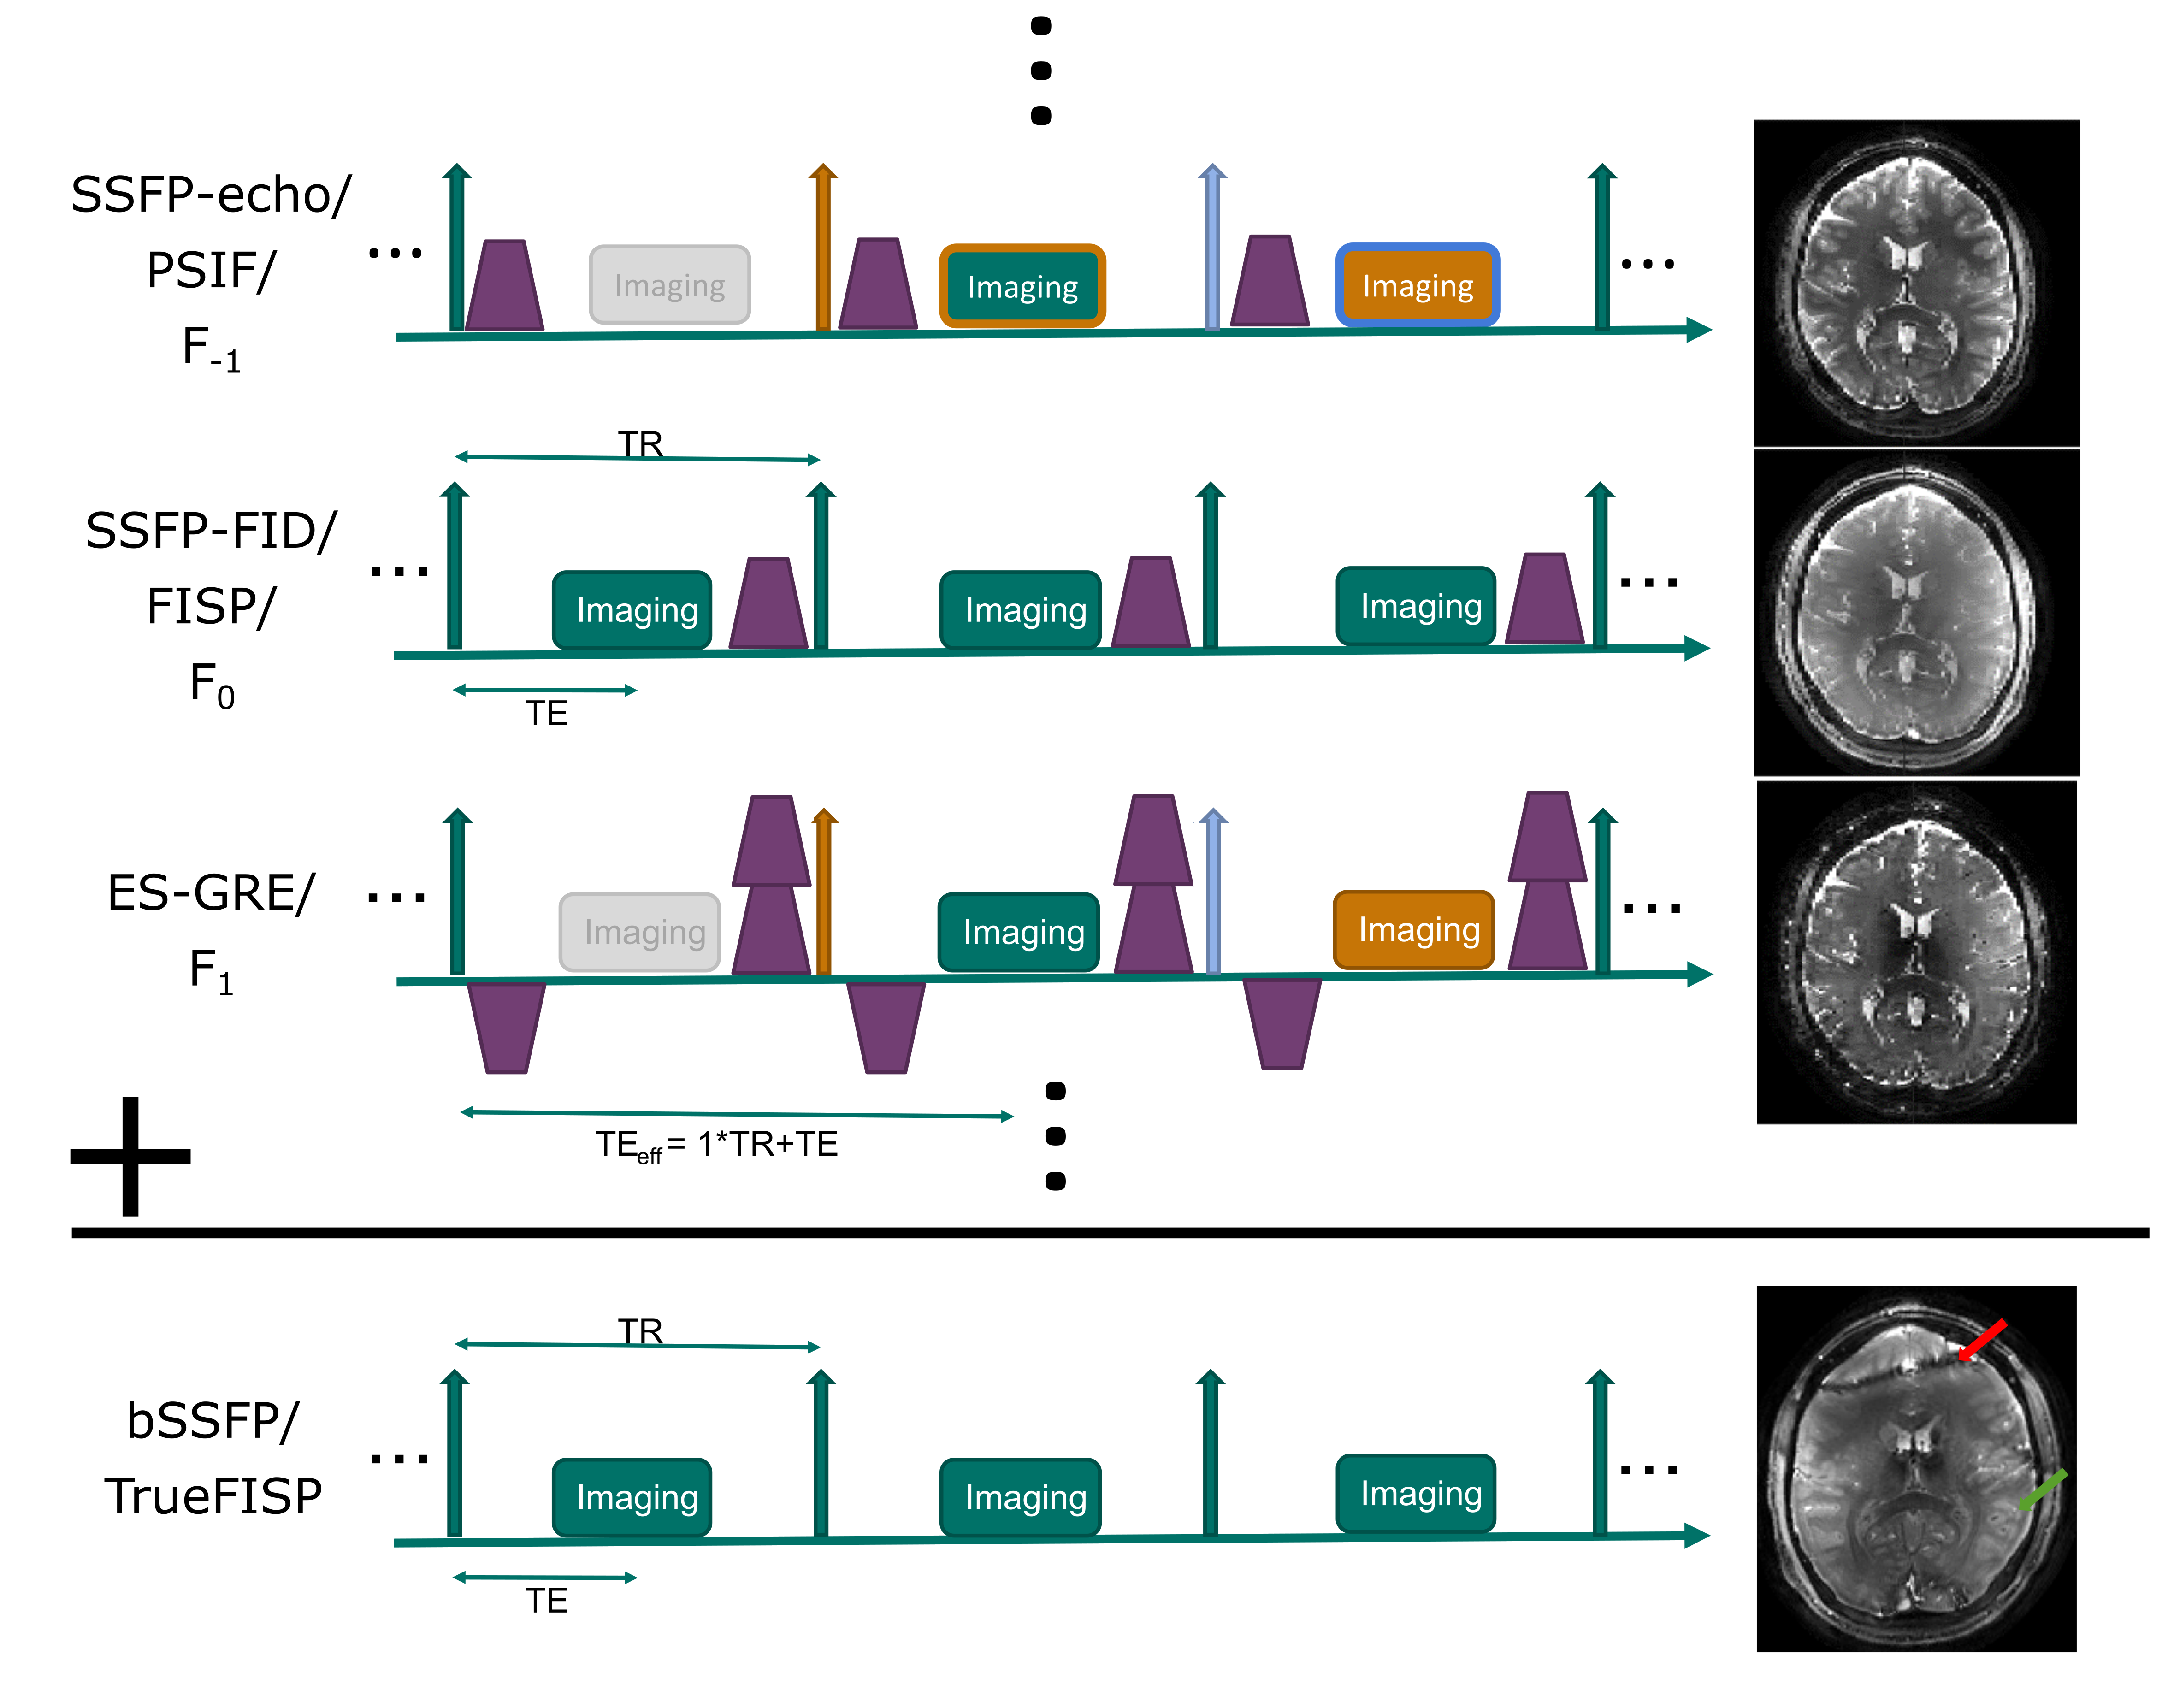
\includegraphics[width=1.0\textwidth]{graphics/bSSFP_echoes.png}
 	\caption{The figure illustrates the \gls{bSSFP} signal, which is a summation of multiple signal pathways. The schematic of the individual non-balanced \gls{SSFP} sequences and the resulting contrast are shown on top. The gradient moments for necessary to achieve $2\pi$ are represented by a purple trapezoidal block. The passband and stopband in the bSSFP contrast image are marked with green and red arrows, respectively.}
 	\label{fig:bSSFP_echoes}
 \end{figure}
 
  Phase cycling enables us to separate the contributions from individual echo pathways \cite{zurMotioninsensitiveSteadystateFree1990}. The transverse magnetization after the RF pulse $M_+$ is given by \cite{zurMotioninsensitiveSteadystateFree1990}
 
 \begin{equation}
 	M^+_{\perp} = \sum_{n=-\infty}^{\infty} A_n e^{jn\theta}
 \end{equation}
 
 where j is $\sqrt{-1}$, $A_n$ is the $n^{th}$ echo amplitude and $\theta$ is the total phase accumulation during each \gls{TR}. In the absence of off-resonance $\vartheta$, phase modulation of the individual echoes can be controlled exclusively with the linear RF phase increment. This allow us to isolate the individual echoes   When the RF increments are equidistant and cover the entire $360^{\circ}$, \gls{DFT} can be used to calculate the echo amplitudes.
 
 \begin{equation}
 	M^+_{\perp}(\Psi) = \sum_{n=-\infty}^{\infty} A_n e^{jn\Psi} e^{jn\Phi}
 \end{equation}
 

\begin{figure}[H]
	\centering
	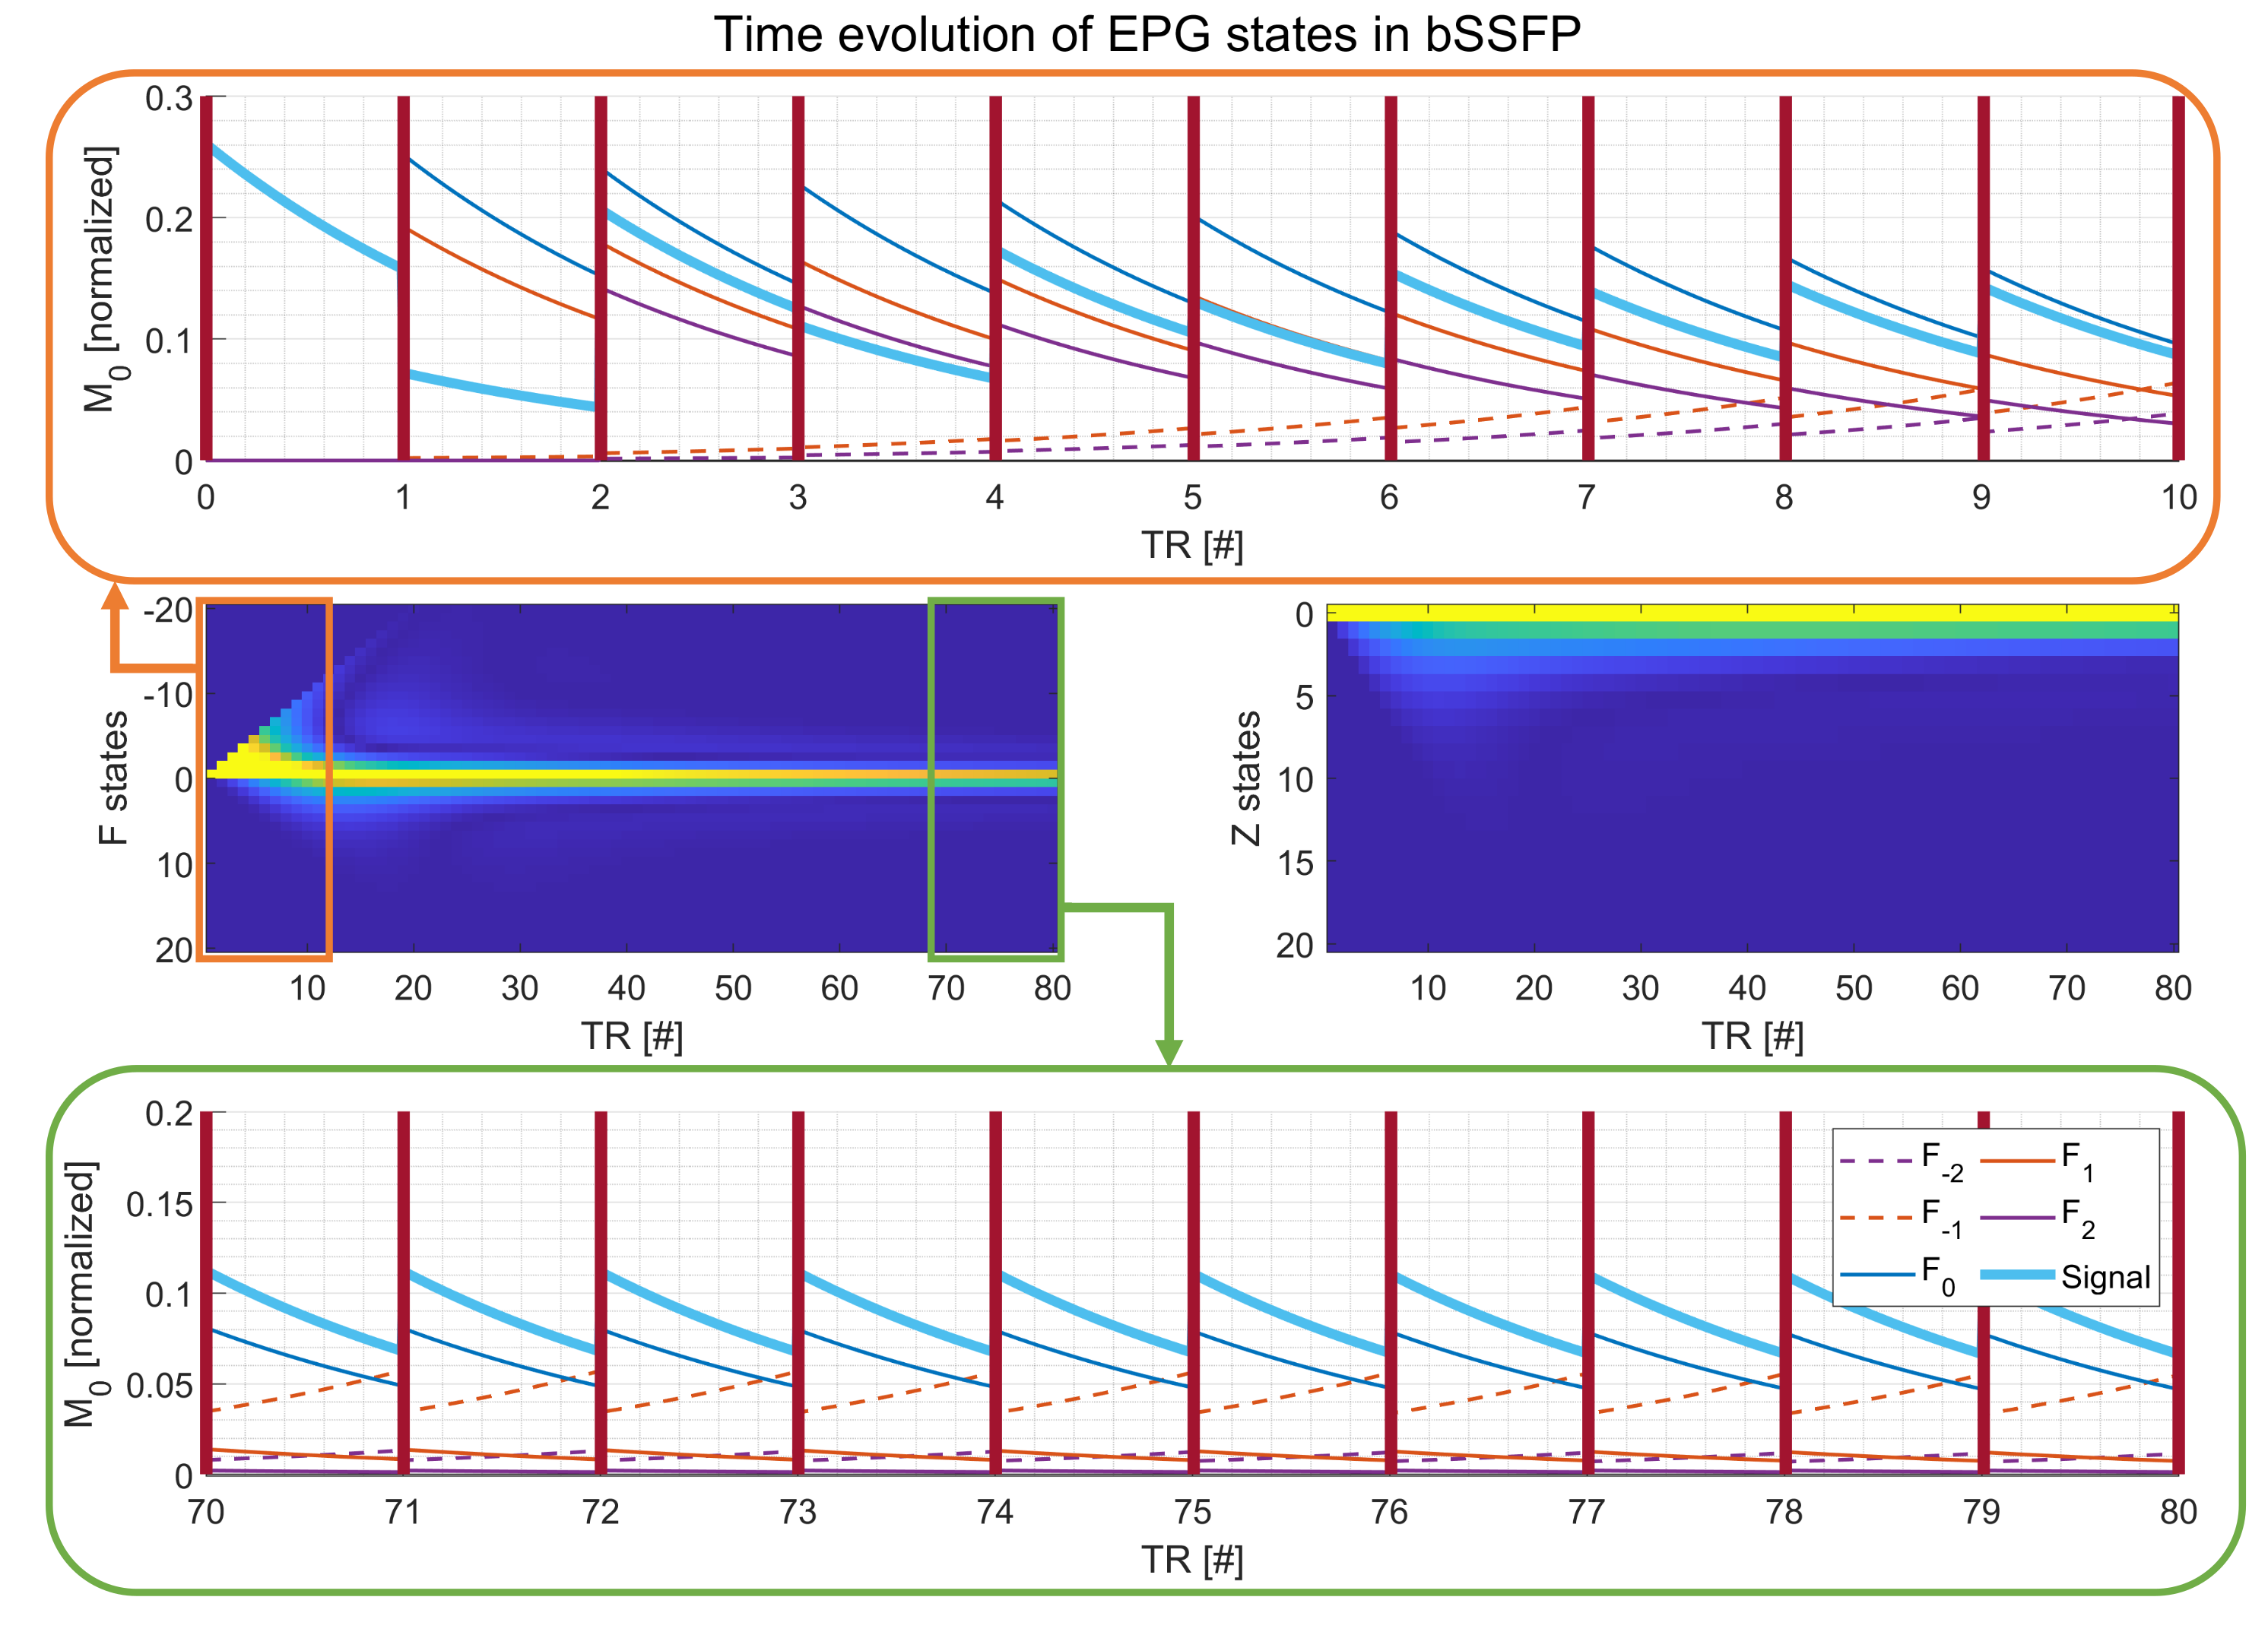
\includegraphics[width=1.0\textwidth]{graphics/bSSFP_EPG.png}
	\caption{Temporal evolution of SSFP configuration modes. The calculated SSFP configuration mode amplitudes with brain grey-matter relaxation times at 9.4 T : $T_1$=2 s and $T_2$=35 ms and sequence parameters: TR=10 ms, flip angle=$15^\circ$ are shown in the middle for 80 repetitions. The first 10 repetitions during the transition and the last 10 }
	\label{fig:bSSFP_EPG}
\end{figure}


thoughts
- in this study, where we used phase graph formalism and why (understand refocusing behavior and simple signal model)
- explain echo pathways
- explain about refocusing and dephasing pathways


\subsection{bSSFP and fMRI}
After the Ogawa et al.\cite{ogawaBrainMagneticResonance1990} reported measuring brain function with susceptibility changes in the blood in 1990, the first \gls{bSSFP} \gls{fMRI} application was reported only in 2001 \cite{schefflerDetectionBOLDChanges2001}. The initial methods\cite{schefflerDetectionBOLDChanges2001,millerFunctionalBrainImaging2003} mainly capitalized on the frequency sensitivity of the \gls{bSSFP} to detect \gls{BOLD} changes in the transition band. In 2005, Bowen et al. \cite{bowenHighFieldBalancedSSFP2005,bowenHighFieldBalancedSSFP2006} reported the first passband bSSFP and suggests its lower sensitivity to large draining veins because of its spin-echo properties\cite{schefflerTrueFISPGradientechoSpinecho2003}. However, the BOLD signal change with \gls{bSSFP} acquisition is only half of that of the GRE-BOLD\cite{schefflerHighresolutionMappingNeuronal2016}. 
